\begin{frame}{SyntheticEddyMethod.jl}
\begin{itemize}
\item \href{https://www.theoj.org/joss-papers/joss.05565/10.21105.joss.05565.pdf}{publication}
\item presented at \textit{JuliaCon2023} at MIT
\end{itemize}

Features:
\begin{itemize}
\item Create fluctuations that respect the divergence-free condition (DFSEM)
\item Create velocity fluctuations for inlet boundary conditions
\item Create coherent eddies in 3D domain
\item Define custom Reynolds Stress Tensor
\item Import from file custom Reynolds Stress Tensor
\end{itemize}
\end{frame}


\begin{frame}{Synthetic Eddy Method}
Reynolds decomposition:
\begin{equation}
    \Vec{u}(\Vec{x},t) = \Vec{U}(\Vec{x},t) +  \Vec{u'}(\Vec{x},t)
    \label{sem:u}
\end{equation}

Compute velocity fluctuations, using a suitable shape function:
\begin{equation}
u_i(\boldsymbol{x})=U_i(\boldsymbol{x})+\frac{1}{\sqrt{N}} \sum_{k=1}^N a_{i j} \epsilon_j^k f_{\sigma(\boldsymbol{x})}\left(\boldsymbol{x}-\boldsymbol{x}^k\right)
\label{sem:ui}
\end{equation}
where $ $ is the shape function (tent, step or Gaussian)
\begin{equation}
    f = 
    \begin{cases}
      \sqrt{\dfrac{3}{2}}(1-|x|) & |x|\leq 1 \\
      0 & |x|>1
    \end{cases}
    \label{sem:tent}
\end{equation}
\end{frame}

\begin{frame}{Synthetic Eddy Method}

    \begin{figure}[h]
        \centering          
        \begin{subfigure}[h]{0.50\textwidth}
                 \centering
            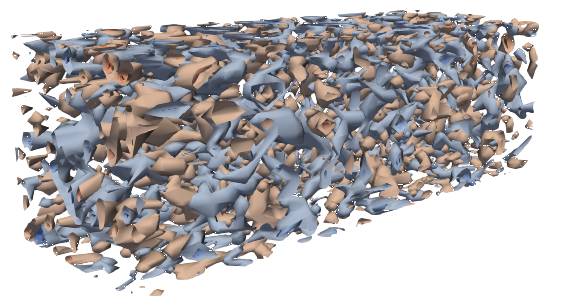
\includegraphics[width=\textwidth]{Isovel.png}
            \caption{Isovelocity contour}

       \end{subfigure}
             \hfill
        \begin{subfigure}[h]{0.45\textwidth}
         \centering
            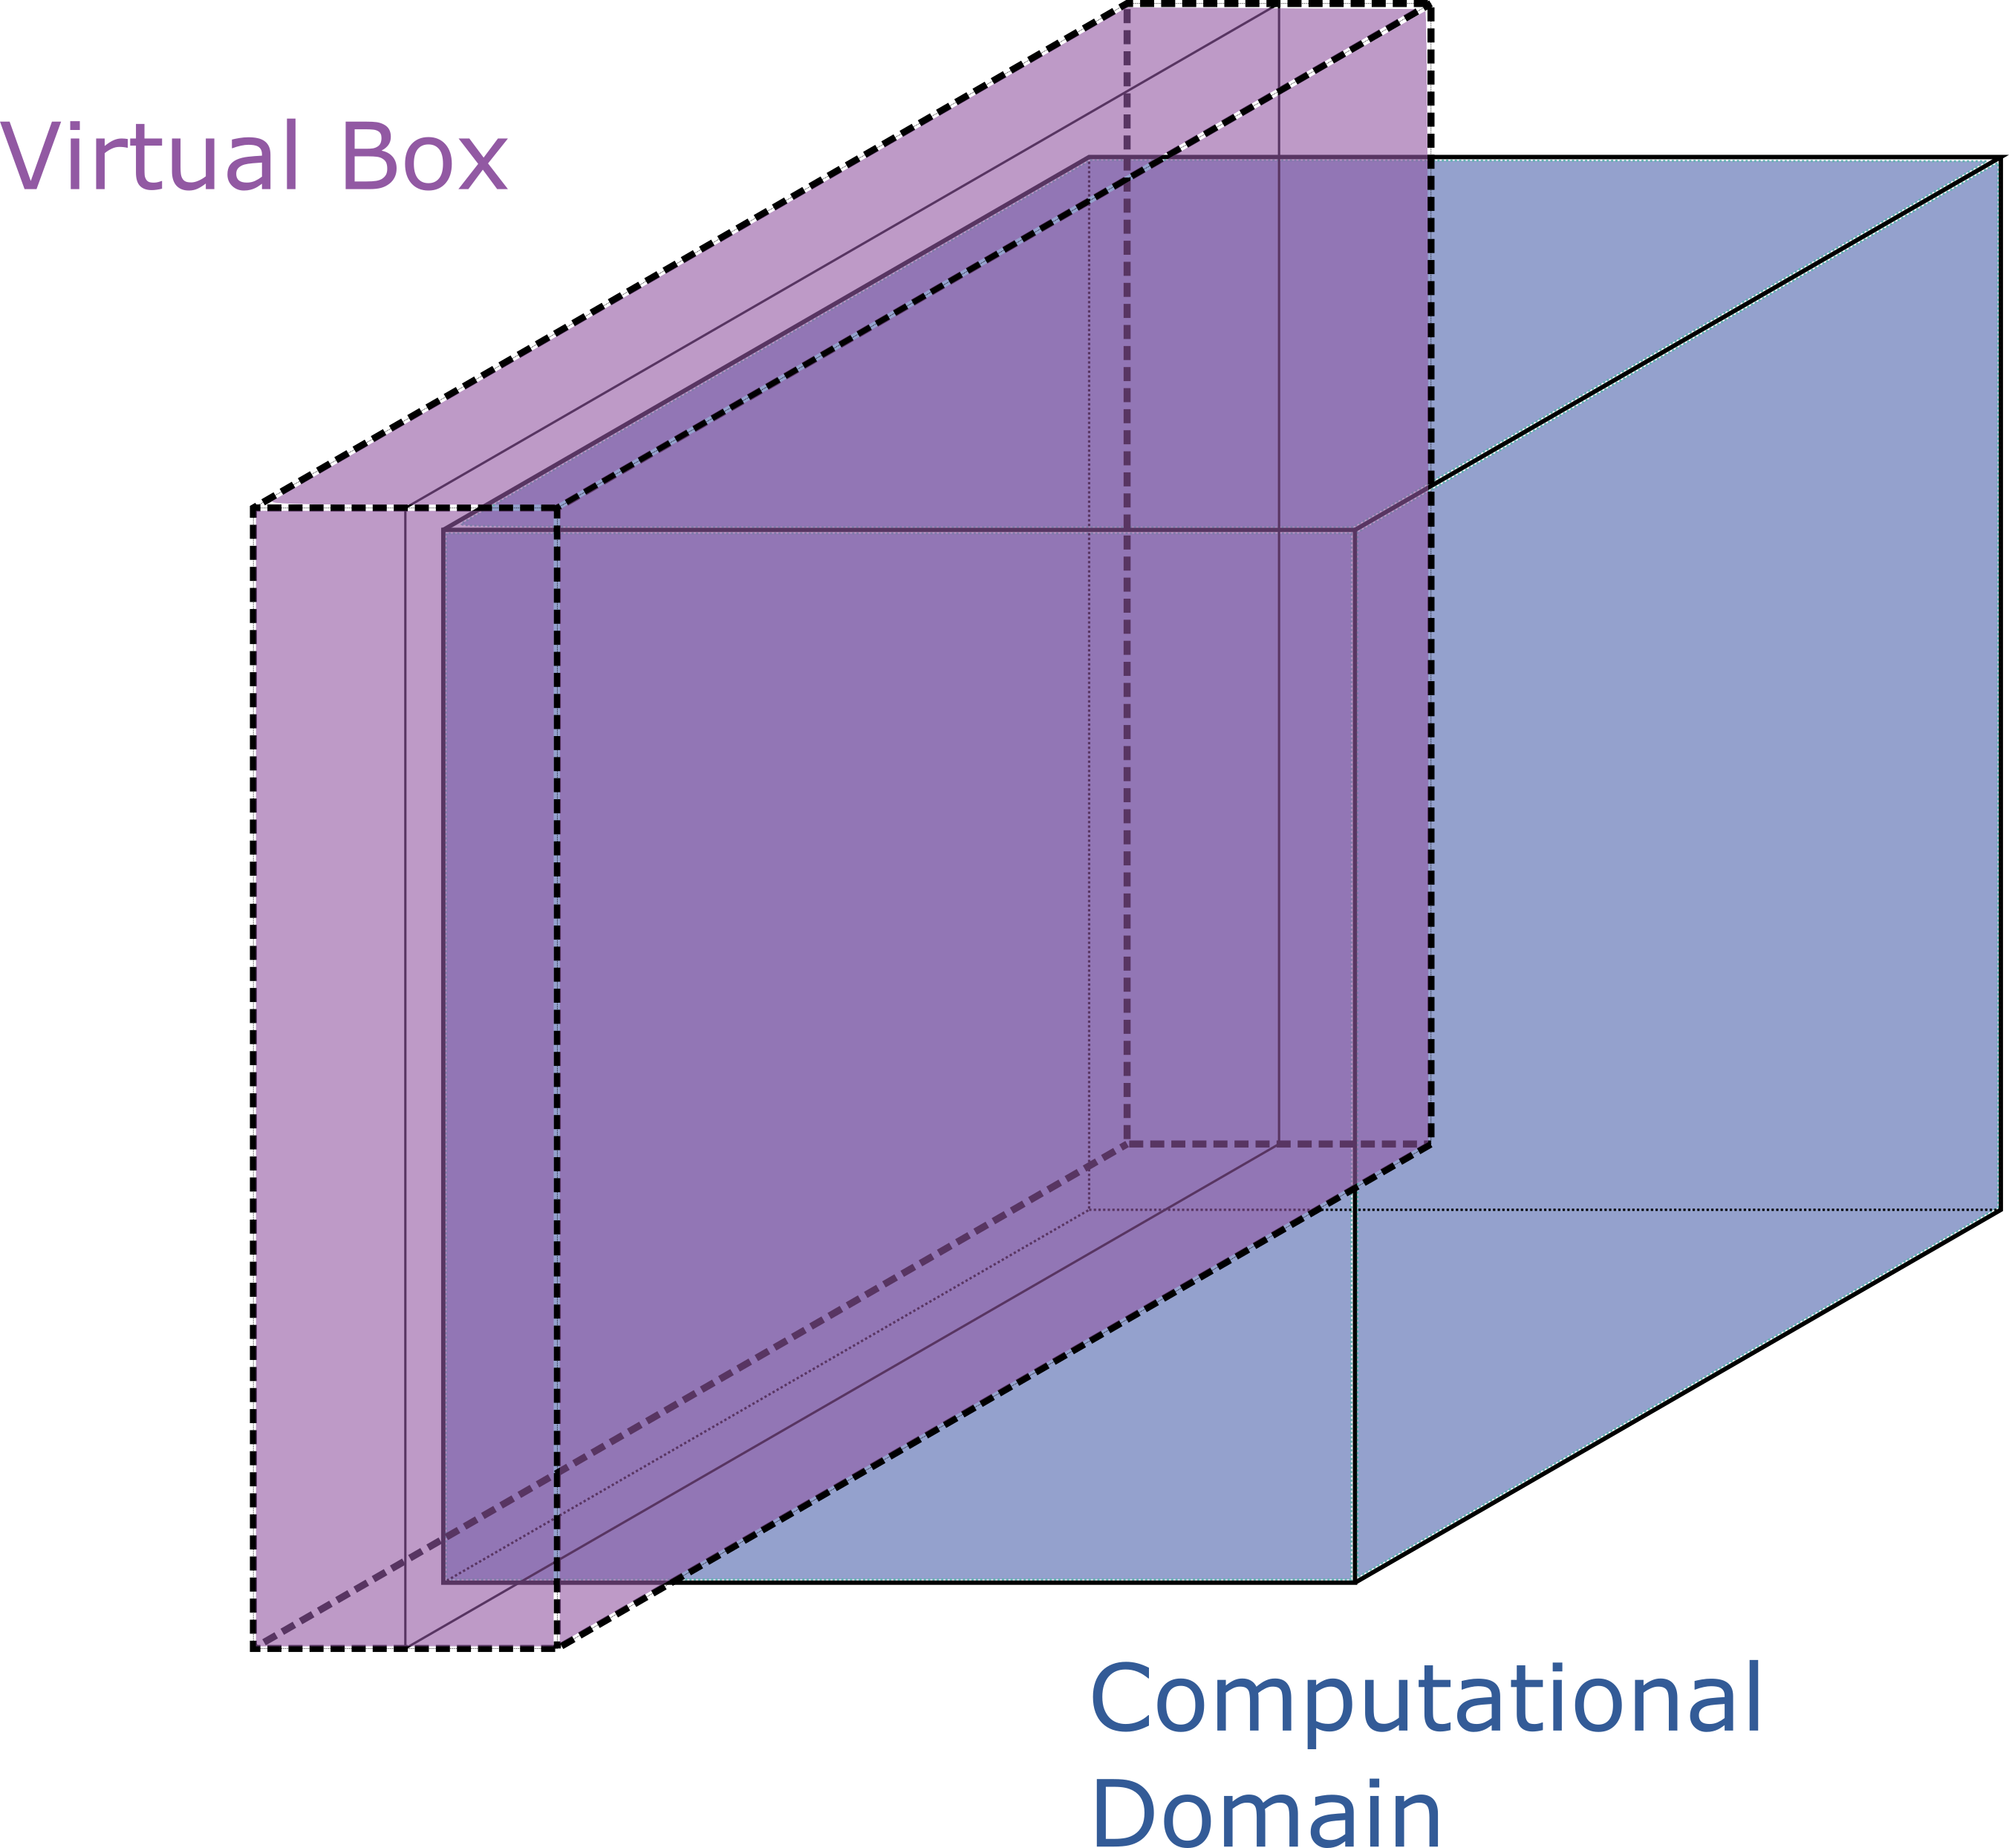
\includegraphics[width=\textwidth]{VirtualBox.png}
            \caption{Virtual Box}

        \end{subfigure}
        \end{figure} 

\end{frame}

\begin{frame}{Synthetic Eddy Method}
    \begin{figure}
        \centering
        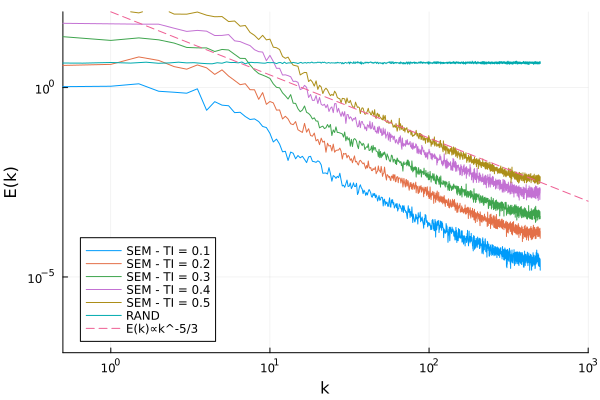
\includegraphics[width=0.65\textwidth]{SEM_vs_RAND_step.png}
        \caption{Power Spectral Density of the turbulent kinetic energy obtained using tent function}
\end{figure} 
\end{frame}
